\section{Einleitung}
In diesem Versuch werden molare Massen mittels zwei verschiedener
Methoden bestimmt.

Einmal mit der Dampfdichtemethode, das andere mal mit der Gefrierpunktserniedrigung.

Zunächst ist als molare Masse das Verhältnis der Masse und der Stoffmenge
definiert,
\begin{equation}
M=\frac{m}{\nu}\frac{g}{mol}\label{eq:Molmasse}
\end{equation}


wobei $\nu$ die Stoffmenge ist und m die Masse.

Ein Mol ist definiert als die Anzahl der Teilchen die in 12g des Kohlenstoffisotops
$^{12}C$ enthalten sind.

Das Molvolumen ist definiert durch das Volumen durch die Stoffmenge
\begin{equation}
V_{m}=\frac{V}{\nu}=\frac{M}{\varrho}\frac{m^{3}}{mol}\label{eq:Molvolumen1}
\end{equation}


V ist das Volumen und $\varrho=\frac{m}{V}$ die Dichte des Stoffes.

Aus der idealen Gasgleichung folgt für eine Stoffmenge von einem Mol.

\begin{equation}
V_{m}=\frac{RT}{p}\label{eq:Molvolumen2}
\end{equation}


R ist die allgemeine Gaskonstante und hat den Wert 8,314$\frac{J}{mol\cdot K}$und
T ist die Temperatur.

Unter Normalbedingungen beträgt das molare Volumen eines idealen Gases
bei einem Mol Stoffmenge etwa 22,41$\frac{l}{mol}$. 

Für eine Stoffmenge von einem Mol ergibt sich für \ref{eq:Molvolumen1}
\begin{equation}
\frac{M}{V_{m0}}=\frac{m}{V_{0}}\label{eq:}
\end{equation}


durch die ideale Gasgleichung bei Normalbedingungen und einigen weiteren
Schritten ergibt sich,
\begin{equation}
M=m\frac{V_{mo}}{V}\frac{p_{0}}{p}\frac{T}{T_{0}}\label{eq:dampfMolMasse}
\end{equation}


diese wird in der weiteren Auswertung gebraucht, m ist die Masse der
Probesubstanz $p_{0}$und $T_{0}$ sind Druck und Temperatur unter
Normalbedingungen.

Da die Probesubstanz mit einer Spritze aufgezogen wird, ist diese
nicht direkt Messbar. Es ist nur die Differenz der Massen der jeweils
gefüllten und leeren Spritzen bekannt.

Es kommt noch ein Zusatzterm hinzu, der dem Auftrieb zu verschulden
ist, somit folgt
\begin{equation}
m=\left(m_{2}-m_{1}\right)+\varrho_{L}V_{Fl}\label{eq:masse}
\end{equation}


$\varrho_{L}$ ist die Dichte der Luft und $V_{Fl}$ das Volumen der
Probesubstanz.

Damit sind die grundlegenden Formeln für die Dampfdichtemethode besprochen,
zur funktionsweise der Apperatur mehr im Versuchsteil.

Bei der Gefrierpunktserdniedrigung wird die molare Masse, durch die
Änderung des Gefrierpunkts eines Stoffes, in dem ein anderer Stoff
in diesem gelöst wird, bestimmt.

Diese wird durch folgende Formel beschrieben,

\begin{equation}
\Delta T=K\frac{1}{m_{L}}\frac{m_{S}}{M_{S}}\label{eq:Temp_diff}
\end{equation}


K heißt kryoskopische Konstante und ist für Lösungsmittel die charakteristische
Größe, in diesem Fall ist das Lösungsmittel Cyclohexan. Hierfür hat
K den Wert $20,2\cdot10^{3}\frac{gK}{mol}$. $m_{L}$ist die Masse
des Lösungsmittels $m_{S}$ die Masse der gelösten Substanz und $M_{S}$ist
die molare Masse der gelösten Substanz.

Diese lässt sich durch einfaches umstellen der Formel berechnen,
\begin{equation}
M_{S}=K\frac{1}{m_{L}}\frac{m_{S}}{\Delta T}\label{eq:molareMasse}
\end{equation}


damit lassen sich die gewünschten Berechnungen durchführen.
%\begin{equation}
%	M = m \frac{V_m}{V}\frac{p_0}{p}\frac{T}{T_0} \label{eq:dampfMolMasse}
%\end{equation}
\newpage
\section{Versuchsteil}
\subsection{Messung der molaren Masse anhand von Dampfdichte}
Im ersten Versuchsteil wird die molare Masse von Ethanol und Cyclohexan bestimmt. Dazu wird genutzt, dass das molare Volumen von idealen Gasen eine konstante ist und sowohl Ethanol als auch Cyclohexan nur geringfügig von diesem Wert abweichen. \\
Es werden geringe Probenmengen von etwa \SI{.1}{\milli\liter} bei Ethanol und \SI{.2}{\milli\liter} bei Cyclohexan mit einer Spritze in einen Glaskolben injiziert. Durch wiegen der Spritze vor und nach dem Injizieren wird die Masse des injizierten Stoffes bestimmt. Die Temperatur des Kolbens wird durch ein kochendes Wasserbad konstant auf etwa \SI{100}{\degreeCelsius} gehalten. Da die Siedepunkte von Ethanol und Cyclohexan, wie Tabelle \ref{tab:propEthanolCyclo} entnommen werden kann, deutlich darunter liegen, gehen diese im Kolben in die gasförmige Phase über. Das so verdrängte Volumen kann abgelesen werden und zusammen mit der Probenmasse die Molmasse bestimmt werden. Durch fünf Messungen pro Stoff wird die Unsicherheit verringert.
\begin{figure}[H]
\centering
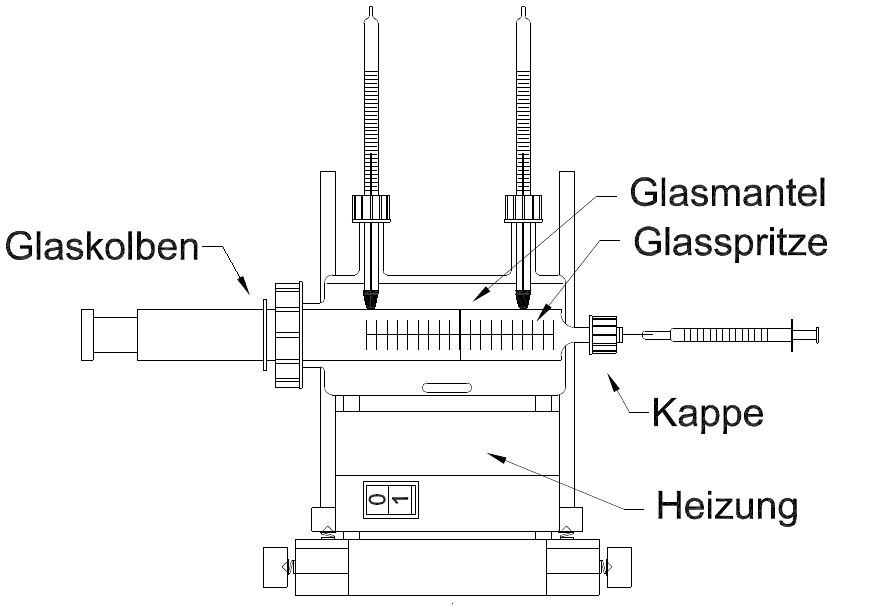
\includegraphics[width=.7\textwidth]{Bilder/aufbau_dampf.png}
\caption[Aufbau]{Versuchsapperatur (Quelle: \cite{anleitung2015})}
\label{fig:aufbau_dampf}
\end{figure}
\subsubsection{Auswertung}

Mit \eqref{eq:dampfMolMasse} lässt sich aus den erfassten Messwerten die molare Masse bestimmen. Da die Formel nur aus linearen und antiproportionalen Zusammenhängen besteht, lässt sich Fehlerformel \eqref{eq:err} verwenden. Der Innendruck des Kolbens passt sich dem Umgebungsdruck an. Daher entspricht $ p $ dem gemessenen Umgebungsdruck $ p = \SI{1001,9(1)}{\hecto\pascal} $. Die Innentemperatur $ T $ war über die Dauer des Experimentes konstant und wurde an beiden Enden gemessen. Die mittlere Temperatur ist $ T = \SI{102,5(8)}{\degreeCelsius} $. Als molares Volumen wird das molare Volumen des idealen Gases von $ V_m = \SI{22.413996(39)}{\mol\per\l} $ angenommen. Dieses gilt bei Normalbedingungen von $ p_0 = \SI{1013,25}{\hecto\pascal} $ und $ T_0 = \SI{0}{\degreeCelsius} $. Die damit bestimmten Ergebnisse sind in den Tabellen \ref{tab:dampf_ethanol} und \ref{tab:dampf_cyclo} zu finden. \\
Die Mittelwerte der molaren Massen betragen \SI{48,3\pm11,7}{\g\per\mol} für Ethanol und \SI{91,9 \pm 15}{\g\per\mol} für Cyclohexan.

\begin{table}[H]
	\centering
	\begin{tabular}{
			S[
				table-figures-integer  = 1,
				table-figures-decimal  = 2
			]|
			S[
				table-figures-integer  = 0,
				table-figures-decimal  = 4
			]|
			S[
			table-figures-integer  = 2,
			table-figures-decimal  = 1
			]}
		{Probenmasse [\si{\g}]} & {Gasvolumen [\si{\l}]} & {Molvolumen [\si{\g\per\mol}]} \\\hline
		0,10 \pm 0,02 & 0,0625 \pm 0,0005 & 49,9 \pm 10,0 \\
		0,13 \pm 0,02 & 0,0825 \pm 0,0005 & 49,1 \pm 7,6 \\
		0,09 \pm 0,02 & 0,0635 \pm 0,0005 & 44,2 \pm 9,9 \\
		0,08 \pm 0,02 & 0,0520 \pm 0,0005 & 48,0 \pm 12,0 \\
		0,13 \pm 0,02 & 0,0805 \pm 0,0005 & 50,3 \pm 7,8 \\
	\end{tabular}
	\caption{Ergebnisse vom ersten Versuch mit Ethanol}
	\label{tab:dampf_ethanol}
\end{table}

\begin{table}[H]
	\centering
	\begin{tabular}{
			S[
				table-figures-integer  = 1,
				table-figures-decimal  = 2
			]|
			S[
				table-figures-integer  = 0,
				table-figures-decimal  = 4
			]|
			S[
				table-figures-integer  = 2,
				table-figures-decimal  = 1
			]}
		
		{Probenmasse [\si{\g}]} & {Gasvolumen [\si{\l}]} & {Molmasse [\si{\g\per\mol}]} \\\hline
		0,24 \pm 0,02 & 0,0765 \pm 0,0005 & 97,8 \pm 8,2 \\
		0,25 \pm 0,02 & 0,0870 \pm 0,0005 & 89,6 \pm 7,2 \\
		0,22 \pm 0,02 & 0,0785 \pm 0,0005 & 87,4 \pm 8,0 \\
		0,14 \pm 0,02 & 0,0510 \pm 0,0005 & 85,6 \pm 12,3 \\
		0,17 \pm 0,02 & 0,0535 \pm 0,0005 & 99,1 \pm 11,7 
		
	\end{tabular}
	\caption{Ergebnisse vom ersten Versuch mit Cyclohexan}
	\label{tab:dampf_cyclo}
\end{table}

\begin{figure}[H]
\centering
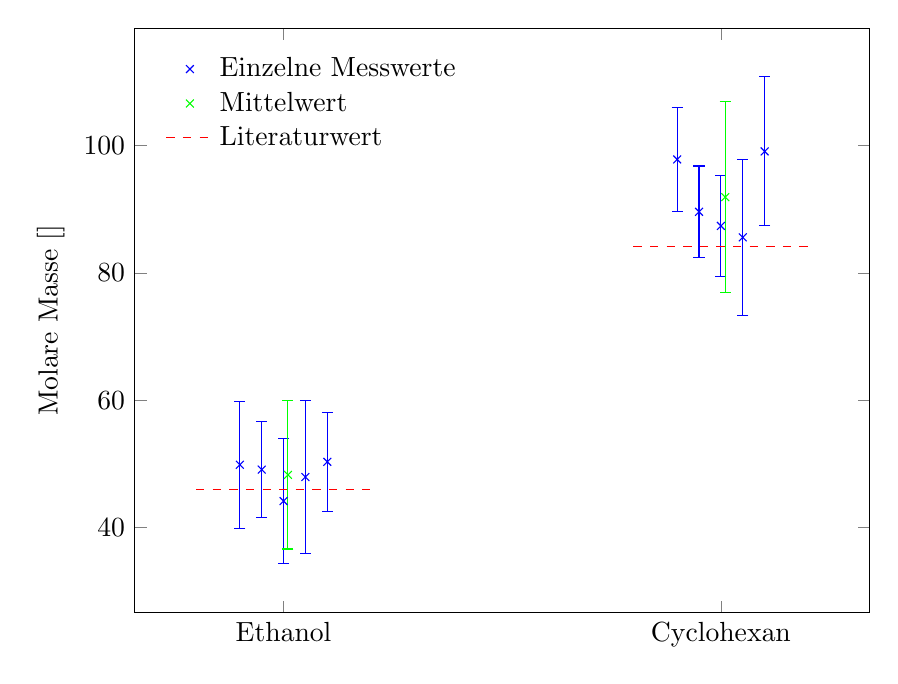
\begin{tikzpicture}
\begin{axis}[width = .9\textwidth, height = 9cm,
	xtick={.3,1.3},
	xticklabels={Ethanol, Cyclohexan},
	ylabel = {Molare Masse [\si{\g\per\mol}]},
	legend style={draw=none, legend cell align = left}, legend pos = north west]

\addplot[blue, only marks, error bars/y dir = both, error bars/y explicit, mark = x] table[x=x,y=y, y error = err] {
x	y	err
.2	49.8785358849	9.9841273896
.25	49.1228004927	7.5637826811
.3	44.1837424177	9.8251242482
.35	47.9601306586	11.9992384215
.4	50.343242741	7.7520048157
};

\addplot[green, only marks, error bars/y dir = both, error bars/y explicit, mark = x] table[x=x,y=y, y error = err] {
x	y	err
.31	48.297690439	11.634048942
};

\addplot[dashed, red, domain=.1:.5] {46.07};

\legend{Einzelne Messwerte, Mittelwert, Literaturwert}

\addplot[blue, only marks, error bars/y dir = both, error bars/y explicit, mark = x] table[x=x,y=y, y error = err] {
x	y	err
1.2	97.8010507547	8.1771956813
1.25	89.5807038163	7.1869095787
1.3	87.3668622188	7.9636160815
1.35	85.5759194104	12.2549480494
1.4	99.0578399583	11.6920686252
};

\addplot[green, only marks, error bars/y dir = both, error bars/y explicit, mark = x] table[x=x,y=y, y error = err] {
x	y	err
1.31	91.8764752317	14.9681458409
};
\addplot[dashed, red, domain=1.1:1.5] {84.16};
\end{axis}
\end{tikzpicture}
\caption{Grafische Darstellung, Quelle Literaturwerte: \cite{wiki:cyclohexan,wiki:ethanol}}
\end{figure}




\subsection{Messung der molaren Masse anhand er Gefrierpunktserniedrigung}

In diesem Teil wird im Lösungsmittel Cyclohexan eine geringe Menge
Eicosan gelöst und der Unterschied der Gefrierpunkte gemessen. Dabei
liegen die Mengen bei $\left(16,27\pm0,02\right)g$ Cyclohexan und
$\left(0,39\pm0,01\right)g$ Eicosan.

Zunächst wurde der Gefrierpunkt des Cyclohexans gemessen. Dafür wurde
die Subtanz in einem Reagenzglas in ein Eisbad gelegt und unter ständigem
rühren abgekühlt. Wird ein Plateau erreicht, wurde der Gefrierpunkt
ermittelt. Dieser liegt bei $T_{1}=\SI{6.6(1)}{\degreeCelsius} $

Die Ermittlung des Gefrierpunkts für das Stoffgemisch aus Cyclohexan
und Eicosan ist analog, nur ist das rühren noch wichtiger als vorher.
Hier liegt der Gefrierpunkt bei $T_{2}=\SI{3.3(1)}{\degreeCelsius}$.

Damit beträgt die Temperaturdifferenz $\Delta T=T_{1}-T_{2}=\left(3,3\pm0,2\right)K$.

Nach (1.8) gilt,
\[
M_{S}=20,2\cdot10^{3}\frac{gK}{mol}\frac{1}{\left(16,27\pm0,02\right)g}\frac{\left(0,39\pm0,01\right)g}{\left(3,3\pm0,2\right)K}
\]


das ergibt,
\[
M_{S}=\left(146,73\pm4,80\right)\frac{g}{mol}
\]


dieser Wert stimmt mit dem Literaturwert von $\SI{282.55}{\g\per\mol}$ (Quelle: \cite{wiki:alkane})
leider nicht überein. 

\section{Diskussion} % !!!!
\subsection{Messung anhand von Dampfdichte}
Zunächst fällt auf, dass die von uns bestimmten molaren Massen innerhalb ihrer jeweiligen Fehler mit den Literaturwerten aus Tabelle \ref{tab:propEthanolCyclo} übereinstimmen. Insbesondere bei der Messung mit Ethanol liegen alle Einzelmessungen und auch der Mittelwert nah am Literaturwert. Beim Cyclohexan dagegen liegt bei zwei der Messungen der Literaturwert nicht im Vertrauensintervall. Dies unterstreicht auch die Wichtigkeit mehrerer Messungen. Die drei anderen Messwerte liegen dagegen deutlich näher an der Referenz.\\
Eine Auffälligkeit der Fehler ist, dass alle bis auf einen Wert zu hoch sind. Als Fehlerursache kommen mit Blick auf die \eqref{eq:dampfMolMasse} eine zu große Masse oder Temperatur oder ein zu kleines Volumen oder zu kleiner Druck in Frage. Da die Temperatur in der Größenordnung \SI{375}{\K} liegt und relativ dazu sehr genau bestimmt werden kann, kann diese nur einen geringen Beitrag zum Fehler haben. Entsprechendes gilt auch für den Druck.
Also ist der Fehler auf Masse und Volumen zurück zu führen. Wahrscheinlich ist bei den Messungen ein Teil der Probe nicht weit genug in den Kolben injiziert worden, so dass diese sich nicht, oder nur langsam erwärmt hat. Dadurch wird ein zu geringes Volumen gemessen und somit eine zu große molare Masse berechnet. Die Probenmasse wurde zwar systematisch falsch gemessen, da der Auftrieb vernachlässigt wurde, jedoch liegt die Dichte von Luft mit $ \rho_L = \SI{1,293}{\kilo\g\per\cubic\meter} = \SI{,001293}{\g\per\cubic\centi\m} $ (Quelle: \cite{wiki:luft}) zwei Größenordnungen unter der von Ethanol und Cyclohexan (siehe Tabelle \ref{tab:propEthanolCyclo}) und kann gegenüber der Messgenauigkeit der verwendeten Waage vernachlässigt werden.
Möchte man eine genauere Messung erreichen sollte man zwei weitere Dinge beachten. Zum einen sollte das oben beschriebene Problem berücksichtigt werden, und sichergestellt werden, dass die gesamte Probe verdampft. Dies kann geschehen indem man sich mit dem Versuch mehr Zeit lässt, oder man die Einfüllvorrichtung optimiert. Zum anderen sollte man die Masse der Probe genauer bestimmen. Rechnet man die Messergebnisse unter Vernachlässigung des Fehlers der Masse aus, so verringert sich der systematische Fehler auf \SI{.4}{\g\per\mol} für Ethanol und \SI{.8}{\g\per\mol} für Cyclohexan. Aber auch die Erhöhung der Messgenauigkeit um nur eine Größenordnung senkt den Fehler um fast eine Größenordnung.

\subsection{Messung anhand von Schmelzpunktverschiebung}

Das Ergebnis für die Gefrierpunktserniedrigung weicht weit vom Literaturwert
ab. Generell wurden alle Messungen korrekt durchgeführt, aber um diesen
Fehler zu erklären muss es an einer Stelle einen groben Fehler gegeben
haben. Die Temperaturdifferenz ist korrekt und das Eicosan war bereits
in 400mg Rationen aufgeteilt, somit ist es wahrscheinlich, dass der
Fehler bei der Menge des Cyclohexans liegt. Wobei zu erwähnen ist,
dass dieser Wert auch im Rahmen liegt. 